\documentclass[a4paper,12pt]{article}

\usepackage{amssymb}
\usepackage{fontspec}

\usepackage{fullpage}
\usepackage{covington}
\usepackage{natbib}

\usepackage{xltxtra}
\usepackage{url}

\usepackage[obeyDraft]{todonotes}
\usepackage{ifpdf}

\usepackage{multirow}

\pagestyle{empty}
%\bibliographystyle{natbib.fullname}
\bibliographystyle{cslipubs-natbib}

\title{Quality and Speed Trade-Offs in
%    Language and Error Models of
    Weighted Finite-State Spell-Checking and Correction}

\author{Tommi A Pirinen\\
 [0.5cm] University of Helsinki\\ % top level affiliation
 Department of Modern Languages\\ % basic academic or research unit
 \texttt{tommi.pirinen@helsinki.fi}}   % email

\date{\today (draft)}

\begin{document}

\maketitle
\thispagestyle{empty}

\begin{abstract} \noindent The following claims are often proposed to support
    Finite-state methods for spell-checking: 1) Finite-state language models
    provide support for the morphologically complex languages that word lists,
    affix stripping and such approaches do not provide (the claim of coverage),
    2) Weighted finite-state models have expressive power equal to the
    state-of-the-art string algorithm spell-checkers (the claim of quality),
    and 3) Finite-state models are at least as fast as string algorithms for
    lookup and error correction (the claim of efficiency).  In this article we
    survey contemporary finite-state spell-checking methods, and perform tests
    in light of these claims to evaluate the current state-of-the-art
    finite-state spell-checking methods.

    To test the claim of coverage, we perform the tests on a range of
    languages with varying morphological complexity: English,
    Northern Sámi and Greenlandic.  To test the claim of quality, we use
    finite-state spell-checking methods that reproduce the current
    state-of-the-art in string-based spell-checking: probability weights for
    word-form and error likelihoods, manual tuning of error probabilities, and
    so forth---in short the full suite of features of spell-checkers like
    Hunspell, as well as the contemporary scientific results. To test the claim
    of efficiency, we use a large scale error corpus acquired from freely
    available and usable open sources. The main goal of this article is thus to
    survey the state-of-the-art in spell-checking and evaluate its
    implementation in finite-state technology.  

    With these tests we verify that it is possible to tune a finite-state
    spell-checking system to outperform the traditional approaches on all parts
    for English spell-checking. We also show that the models for
    morphologically complex languages are on par with the English system with a
    few simple considerations. We go through the parameters that need to
    be considered when tuning the system for performance and quality.

\end{abstract}


\makeatletter\let\chapter\@undefined\makeatother
\listoftodos

\section{Introduction} 

Spell-checking and correction is a traditional and well-researched part of
computational linguistics. Specifically, spell-checking and
correction with finite-state automata is one of the more recent branches in the
effective spell-checking of typologically varied languages. Finite-state
methods for language models are widely recognised as a good way to handle the
morphologically more complex languages~\cite[]{beesley2003finite} in a similar
manner as the isolating languages---as far as recognising the correct
word-forms is concerned. One of the simplest example of this is that a
finite-state automaton can encode dictionaries of infinite size, which is a
common need for languages with productive derivational and compounding
phenomena.  In these cases a simple word-list lookup has often proved
insufficient. The principal contribution of this article is to survey the use
of different weighted, fully finite-state spell-checking systems for
morphologically complex languages that have not been implemented with
word-list spelling checkers.  We survey the existing finite-state models and
some non-finite-state models that can be easily implemented in finite-state
form.  As the set of the languages, we have selected to study North Sámi from
the complex, agglutinative group, Greenlandic from complex poly-agglutinative
and English to confirm that our finite-state formulations of traditional
spelling correction applications are working as described in the literature.

Furthermore, as contemporary spell-checkers are increasingly using statistical
approaches to the task, the weighted finite-state models provide the equivalent
expressive power, even for the more complex languages by encoding the
probabilities as weights in the automata.  The same applies to the error
models. As the programmatic noisy channel models~\cite[]{brill2000improved} can
encode the error probabilities when making the corrections, so can the weighted
finite-state automata encode these probabilities. This article goes through the
methods that are used to encode the probabilities into weighted finite-state
language and error models, and evaluates them on large-scale testing material.

The task of spell-checking is split into two parts, error detection and
correction. In the error detection task, the purpose is to locate the words to
be corrected, e.g. to determine that \emph{cta} is not an English word in text
when \emph{cat} is. In literature this is often described as looking up the
words from a dictionary or a word list, which is nearly accurate for the means
of this article as well. In our case though, the word list is substituted with
a finite-state automaton, and on a more abstract level we refer to this as
\emph{language model}, rather than word list. The additional point that is
relevant to morphologically complex languages is that a language model should
cover the infinite lexicons of our target languages, so we might for
example detect that the word \emph{purppura-apinatiskikone} (purple monkey dish
washer) is a plausible word in the Finnish language even though it is not in a
dictionary nor any corpora.

Error detection by language model lookup is referred to as \emph{non-word} and
\emph{isolated} error detection. More complex error detection systems may be
used to detect words that are correctly spelled, but are unsuitable in the
context based on syntax or semantics. This is referred to as \emph{real-word}
error detection \emph{with context} \cite{mays/1991}.

The implementation of error detection using a context-sensitive finite-state
system is plausible based on e.g. the approach of~\cite{silfverberg/2010},
which presents a finite-state implementation of an n-gram model with reasonable
speed. The task of detecting isolated errors from the text is often considered
trivial or solved in many research papers dealing with spelling correction
\cite[e.g.][]{otero/2007}; precision and recall are directly dependent on
dictionary size and improvement is a simple process of adding words.  There is
a small trade-off in rare cases where a common word misspelt will become a very
rare word (e.g. \emph{minuets} instead of
\emph{minutes}~\cite{kukich1992techniques}). The approach to this, as well as
the problem of detecting real-word errors, is the application of statistical
context-based models.  However, this is already more problematic since there is
direct trade-off in precision versus recall depending on likelihood cut-off
\cite[]{hirst2008evaluation,wilcoxohearn2008realword}.

The task of error-correction is the task of generating the list of the most
likely correct word-forms given the misspelled word-form that was located in
spell-checking process. The method of correction is often referred to as an
\emph{error model}. This alludes to our practical implementation in which the
error correction task is implemented by simulating the process of making errors
as a finite-state model. The main point of this error modeling is to correct
spelling errors accurately by observing the causes of errors and making
predictive models of them~\cite[]{deorowicz2005correcting}.  This modeling
effectively splits the error models into numerous sub-categories, each
applicable for correcting specific types of spelling error; the most used and
common model is accounting for the mistypings, that is, the slips of fingers on
the keyboard. This model is nearly language agnostic, although it can be tuned
to each local keyboard layout. The other set of errors is more language
specific and user specific---it stems from the lack of knowledge or language
competence, e.g.  in the non-phonemic orthographies, such as English, the
learners and the unskilled writers commonly make mistakes like writing
\emph{their} instead of \emph{there} since they are pronounced alike; similarly
competence errors will give rise to the common confusables in many languages,
like missing an accent, writing some digraph instead of its unigraph variant,
or confusing some morph with another.

There are two main finite-state approaches to the task of ranking the
correction suggestions studied in this article; using the probabilities given
by the language model for the word-forms that are correct, and using the
probabilities given by the error-correcting model for the likelihood of the
user typing the specific misspelling when meaning the corrected form, i.e. the
likelihood of the user making a specific series of errors. This article surveys
the existing weighted finite-state methods for creating these two probabilistic
models and combining them. One note should be made when thinking of the error
correction, the application of the error model is not independent of the type
of the errors detected, and these two components can be kept fully apart; an
error model that corrects non-word errors will come up with (possibly
suboptimal) suggestions in context, and an error model tuned for real word
errors will correct non-word errors as well.

One of the recent themes in research into finite-state spell-checking and
correction is using the weighted finite-state automata to improve the precision
or the accuracy of spelling correction---and even the checking---methods.
What is problematic with the combination of these methods and language models,
is that they require large amounts of data. To train the language models one
would expect to have corpora where at least a majority of correctly spelled
word-forms are available.  For polysynthetic languages, like Greenlandic, even
a gigaword corpus, would not usually be nearly as complete as an English corpus
with a million word-forms. To cope with the resource-poor morphologically
complex languages in situations like this, we study a few of the more
advanced linguistically motivated corpus training methods, like compound
part~\cite[]{pirinen/2009/nodalida} or morpheme weighting schemes and study
their effects.

One common source of the probabilities for ranking the suggestion is the
neighboring words and word-forms \cite[]{pirinen2012improving,otero/2007}.  In
this survey we explore the limitations of this kind of context-language model
in terms of speed and size with respect to the amount of improvement they
present for morphologically complex languages and contrast it with the
traditional results for morphologically isolating languages
\cite[]{mays/1991,wilcoxohearn2008realword}.

Another aspect of resource-poor languages is that more advanced language model
training schemes, such as the use of morphological analyses as error detection
evidence~\cite[]{mays/1991} and a factor in correction
ranking~\cite[]{otero/2007}, would require large \emph{manually verified}
\emph{morphologically analysed} and \emph{disambiguated} corpora, which simply
do not exist as open, freely usable resources, if at all. The same problem on a
smaller scale applies to improving the error correction models with data from
the error corpora; the corpus should contain both the errors and right
corrections for better results. For this reason we concentrate here on showing
what kind of improvement can be made with smaller, obtainable corpora
accompanied with hand-crafted rules approximating the lacking
\emph{probabilities}.

This article is structured as follows: In the following
Subsection~\ref{subsec:background} we describe the history of spell-checking up
to the finite-state formulation of the problem, then show the traditional
finite-state approaches to the problem, and describe how our weighted
finite-state implementation compares with the other applications presented in
the literature.  In Subsection~\ref{subsec:theory} we briefly revisit the
notations and assumptions behind the statistics we apply to our language and
error models.  In Section~\ref{sec:methods} we present the popular methods of
creating finite-state language and error models for the spell-checkers,
describe getting the probabilities or similar weights into the finite-state
spell-checker, describe the methods of inducing weights into the language and
error models, the methods of creating the weighted language and error models
from data, and finally the methods of combining the weights of the different
sources of data and probabilities. In Section~\ref{sec:material} we present the
actual data, the existing language models, the error models and the corpora we
have used, and in Section~\ref{sec:evaluation} we show how the different
combinations of the languages, the weighing schemes and the error models affect
the accuracy and the precision, and the speed of the finite-state
spell-checking. In Section~\ref{sec:discussion} we discuss implications of
our results with regards to previous findings and lay out the possible future
extensions and solutions, and finally, in Section~\ref{sec:conclusion} we
conclude our findings.

\subsection{A Brief History of Automatic Spell-Checking and Correction}
\label{subsec:background}

Automatic spelling correction by computer is in itself, an old invention, with
the initial work done as early as in the 1960's. Beginning from the invention
of the generic error model for typing mistakes, the Levenshtein-Damerau
distance \cite[]{levenshtein/1966,damerau/1964} and the first applications of
the noisy channel model~\cite[]{shannon/1948} to
spell-checking~\cite[]{raviv/1967}.  The early solutions treated the
dictionaries as simple word lists, or later, word-lists with up to a few
affixes with simple stem mutations and finally some basic compounding
processes. The most recent and widely spread implementation of this
implementation with a word-list, stem mutations, affixes and some compounding
is Hunspell\footnote{\url{http://hunspell.sf.net}}, which is still in common
use in the open source world of spell-checking and correction.  It is therefore
used as the reference implementation when we describe the methods of the
contemporary spelling checkers in Section~\ref{sec:methods}. The word-list
approach, even with some affix stripping and stem mutations, has sometimes been
found insufficient for the morphologically complex languages.  E.g. even some
recent attempts to utilise Hunspell for Finnish have not been successful
\cite[]{pitkanen/2006}. And in part, the popularity of the finite-state methods
in computational linguistics seen in the 1980's was driven by a need for the
morphologically more complex languages to get language models and morphological
analysers with recurring derivation and compounding processes
\cite[]{beesley2004morphological}.  In this light it is quite surprising, that
many of the recent approaches for finite-state spell-checking are still
concentrating on using acyclic finite-state automata (i.e. the equivalent of
word list) to perform
spell-checking~\cite[]{watson2003new,deorowicz2005correcting}. While this
approach has additional performance, the possibility to use arbitrary
finite-state automata as language models comes without any measurable
modifications to the code~\cite[e.g.][]{pirinen/2010/lrec} and leaves the
option to optimise to the lexicographers, as they can then select to use
acyclic, suffix-tree or regular automaton models.

Given the  finite-state representation of the dictionaries and the expressive
power of the finite-state systems, the concept of the finite-state based
implementation for spelling correction was an obvious development. The
earliest approaches presented an algorithmic way to implement the finite-state
network traversal with error-tolerance \cite[]{oflazer/1996} in a fast and
effective manner \cite[]{agata/2002,hulden/2009}.  In \cite{schulz/2002} the
Levenshtein-Damerau distance was presented in a finite-state form such that the
finite-state spelling correction could be performed using the standard
finite-state algebraic operations with any existing finite-state library.
Furthermore in e.g.  \cite{pirinen/2010/lrec} it has been shown that the
weighted finite-state methods can be easily used to gain the same expressive
power as the existing statistical spell-checking software algorithms.

\subsection{Notations and a Bit of Statistics for Language and Error Models}
\label{subsec:theory}

In this article, where the formulas of finite-state algebra are concerned, we
assume the standard notations from \cite{aho2007compilers}: a one-tape
finite-state automaton $M$ is a system $(Q, \Sigma, \delta, Q_s, Q_f, W)$,
where $Q$ is the set of states, $\Sigma$ the alphabet, $\delta$ the transition
mapping of form $Q \times \Sigma^t \rightarrow Q$, where t is number of tapes
in the automaton, $Q_s$ the initial states of the automaton and $Q_f$ the final
states of the automaton. For weighted automata we extend as in
\cite{mohri2009weighted} such that $\delta$ is extended to $Q \times \Sigma^t
\times W \rightarrow Q$, where $W$ is the weight, and additionally the system
includes a final weight mapping $\rho: Q_f \rightarrow W$. The structure we use
for weights is systematically the tropical semiring $(\mathbb{R}_+ \cup
{+\infty}, min, +, +\infty, 0)$, i.e. weights are positive floats that are
collected by addition.

For the finite-state spell-checking we use the following common notations:
$M_d$ is a single tape weighted finite-state automaton used for detecting the
spelling errors, where threshold $w_d$ may be used to discard bad word forms,
$M_s$ is a single tape weighted finite-state automaton used for suggesting
correct words, where the weight value is used to rank the suggestions.  In many
occasions we study the possibility of $M_d = M_s$. The error models are
weighted two tape automata commonly marked as $M_e$.

In where the probabilities are used, the basic formula to get probabilities
from the discrete frequencies of events (word-forms, mistyping events, etc.) is
straightforward $P(x) = \frac{c(x)}{\mathrm{corpus size}}$, where x is the
event, c is the count or frequency of the event, and corpus size is the sum of
all event counts in the training corpus. The encoding of weights in a
finite-state automaton is done by setting $Q_{\pi_x} = -\log P(x) \in \rho$.
As events not appearing in corpora should have a larger probability than zero,
we use the simple additive smoothing techniques, setting $P(x) = \frac{c(x) +
\alpha}{\mathrm{corpus size} + (\mathrm{dictionary size} \times \alpha)}$, so
for unknown event $\hat{x}$ the probability will be counted as if it had
$\alpha$ appearances.  Another approach would be to set $P(\hat{x}) <
\frac{1}{\mathrm{corpus size}}$, which makes the probability distribution leak
but may work under some conditions \cite[]{brants2007large}.  The interesting
values with this probabilistic weighting is setting threshold $w_d :=
\frac{\alpha}{\mathrm{corpus size} + \mathrm{dictionary size} \times \alpha}$
to filter singleton events e.g. hapax legomena from the training data.

\subsection{Morphologically Complex Resource-Poor Languages}
\label{subsec:morphologically-complex}

One claim examined in this article is that there is a set of morphologically
complex languages for which the finite-state models are a necessity in order to
deal with spell-checking in a manner that is usable for end-users of the
application.  The topic of morphological complexity and linguistic typologies
is wide and the terminology is not generally agreed on, instead of going into
details of the terminology, we show figures related to computational linguistic
properties to demonstrate the practical meaning of computationally
morphologically complex language and why it requires a finite-state approach
instead of plain word lists. With spell-checkers, the important figures for
end-users are coverage---how many valid words the spell-checker recognises out
of all words in the corus---and precision---how many real words the
spell-checker will accepts out of all words it covers.  We relate this to the
question of morphological complexity and computational models by looking at the
size of word-form lists required to have high enough coverage and precision for
the spell-checker. The hypothesis is that languages that are morphologically
complex are capable of producing infinite word-forms via morphological
processes like compounding and derivation, and the number of word-forms covered
by a basic dictionary and inflections is much higher than for English, we base
this hypothesis on the fact that the English inflectional morphology contains
approximately 2 word-forms per dictionary word, so a dictionary of 100,000
words can be covered by word-list of 200,000 word-forms, conversely e.g.
Finnish inflectional morphology is approximately 4,000 word-forms per
noun\footnote{2 number suffixes times 15 cases times 5 possessive suffixes
times 26 combinations of focus clitic particles, give or take a few
allomorphs}, so to approximate the same coverage as English dictionary of
100,000 words is 400,000,000 word-forms, ignoring the productive derivation and
compounding.

We briefly and informally measured from the source texts Wikipedia following:
words collected from first 90~\% of the English Wikipedia will cover 98.9~\%
of the rest of the wikipedia, for North Sámi this number is 65.8~\% and for
Greenlandic 91~\%, in this experiment we did not consider the correctness
of the word-forms, we merely show the extent and shape of the long tail. For
correctness figures related to the productivity of the morphologically
rich languages, we made an experiment measuring coverage with a dictionary
that simulates word-form list by disallowing compounds and derivations, the
results for North Sámi are that without compounds and derivation the
coverage of Wikipedia with the available dictionary is just 1~\% whereas
otherwise it is 48~\%---figures detailed in Section~\ref{sec:evaluation}.

To get another view of the scarcity of the language resource data in terms
of naïve unigram models, in the Figure~\ref{fig:forms-vs-tokens}, we show the
histogram of wikipedia data in terms of how many unique word-forms we get by
reading how many words of wikipedia, this is directly relevant to the
predictive power of such simple unigram model.

\begin{figure}
    \centering
    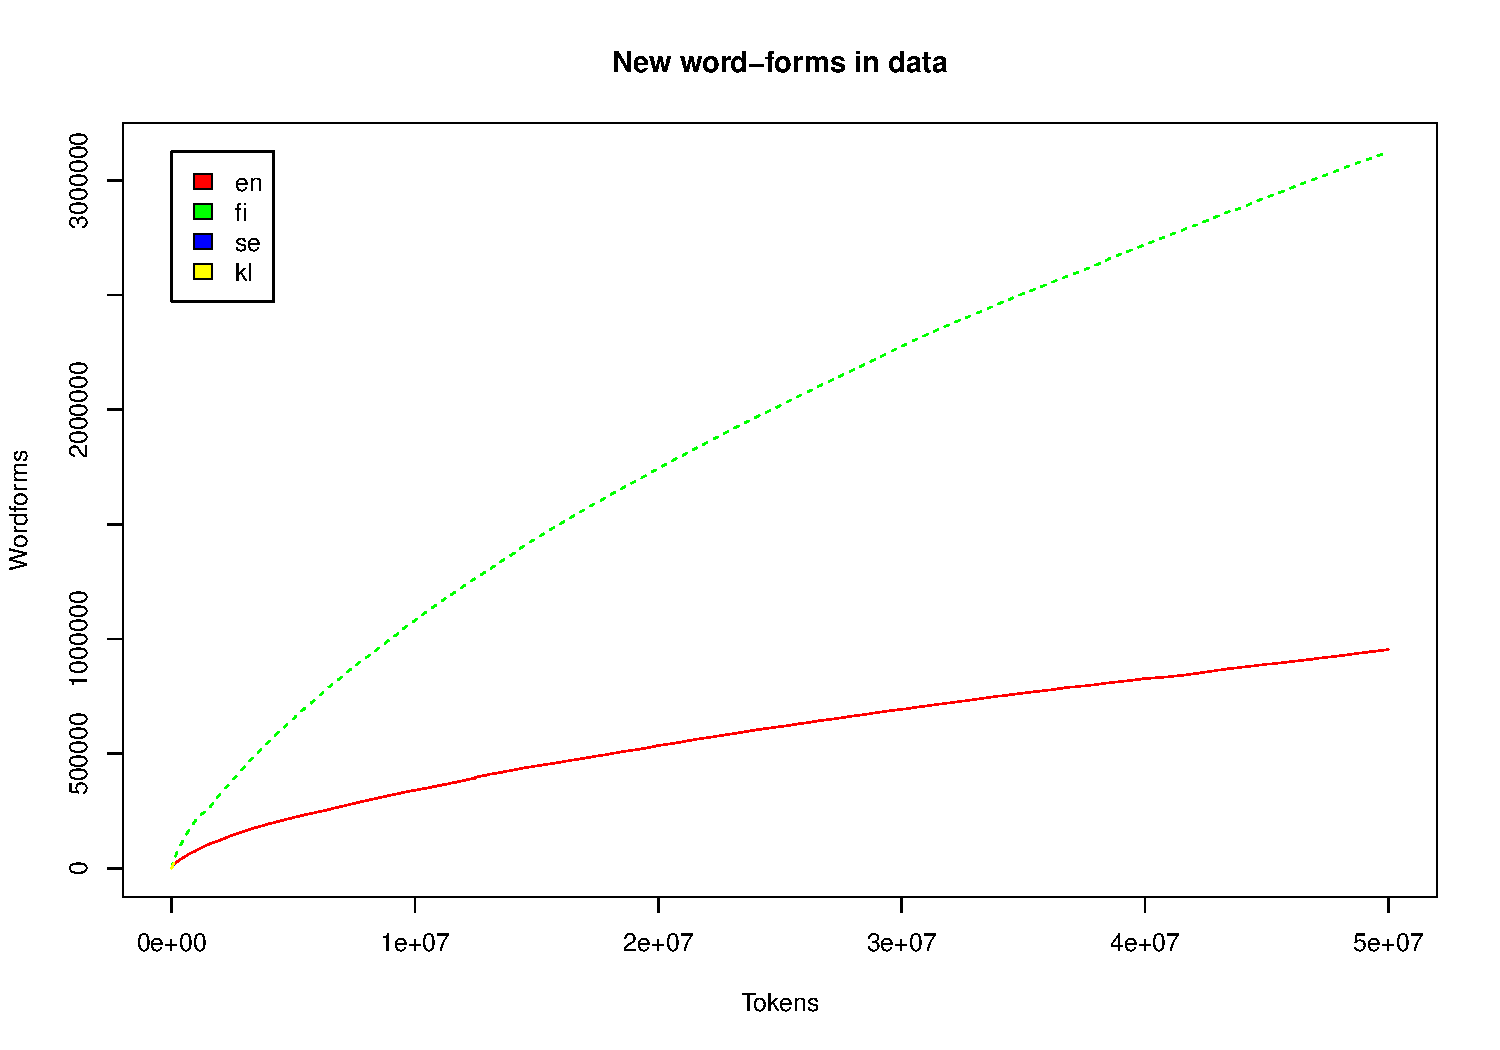
\includegraphics[width=\textwidth]{graphicx/formspertokens}
    \caption{Unique word-forms (y-axis) per tokens (x-axis)
    \label{fig:forms-vs-tokens}}
\end{figure}

\section{Contemporary Methods for Making Finite-State Language and Error Models
and Their Weighting}
\label{sec:methods}

The task of spell-checking is divided into locating the spelling errors and
suggesting the corrections for the spelling errors. In the finite-state
spell-checking the former task requires a language model, that can tell whether
or not a given string is correct. The simplest finite-state approach for this
is just an unweighted single-tape finite-state automaton where all of the
strings recognised by the automaton are considered correct. It is also possible
to use a two-tape automaton where information encoded on the second level aids
in deciding whether the string should be accepted under the current settings
(e.g.  with offensive or sub standard language), and also a weighted
finite-state automaton with a threshold of considering very rare or unusual
words as errors.  This approach is usually taken with context-sensitive
applications~\cite[]{otero/2007}. The error correction requires a language
model, which may or may not be the same for error detection, and an error
model.  The language model for spelling correction, like the one for error
detection, is in the simplest case just an unweighted finite-state automaton
encoding the correct strings of a language. In the case of correction however,
even a very simple probabilistic weighting using a small corpus of unverified
texts will improve the quality of suggestions~\cite[]{pirinen/2010/lrec}, so
having a weighted language model is usually a good thing. Another difference
between a spell-checking language model and a correction model in many
practical applications is, that typically the checker can be much more
permissive with the offensive words, the unlikely derivations, and the
compounds. With regards to suggestions, it is often a wanted feature \emph{not}
to have spelling corrector suggest these offensive or obscure word-forms as
corrections. It is likely, that with the probabilistic data, these forms will
get a low probability and appear towards the end of the suggestion list. The
error modeling part of the error correction is made with a two-tape
finite-state automata, that can encode the relation between misspellings and
the correctly typed words. This relation can also be weighted with the
probabilities of making specific mistypings or errors or just arbitrary
penalties, as is basically done with many of the traditional software-based
approaches \cite[such as][]{hunspell/manual}.

This chapter is organised as follows, in the
Section~\ref{subsec:language-models} we describe how the finite-state language
models are made and how they can be tuned for spell-checking use, as well as
the basic probabilistic and hand-written weighting techniques that have been
used to implement the weighted language models in finite-state context. In
Section~\ref{subsec:error-models} we go through a number of popular schemes for
modeling the typos and other spelling errors.  In
Section~\ref{subsec:manual-weighting} we go through some finite-state weighting
schemes that are based on mainly the expert judgement and fiddling with the
weights.  In Section~\ref{subsec:automatic-weighting} we study the methods for
inducing the weights for the language and the error models from unannotated and
small annotated corpora, and in Section~\ref{subsec:combining-weights} we show
both statistically sound and unsound methods of combining the weights in the
models.

\subsection{Compiling Finite-State Language Models}
\label{subsec:language-models}

The baseline for any language model as realised by numerous
spell-checking systems and a the literature is a word-list (or a word-form
list). One of the most popular example of this approach
is \cite[]{norvig/2010} describing how he programmed a toy spelling corrector
during an intercontinental flight. The finite-state formulation of
this idea is equally simple; given a list of word-forms we compile each string
as a path in an automaton \cite[]{pirinen2012effects}. In fact, even the
classical optimised data structures used to efficiently encode word lists, like
tries and acyclic deterministic finite-state automata are usable as
a finite-state automata for our purposes without modifications.

Moving to more advanced word lists, such as the affix stripping and stem
mutating ones of hunspell, the finite-state formulation becomes slightly more
complex, but the basics are the same: the roots are a disjunction of string
paths and so are the affixes. The correct morphotactic combinations and the
stem mutations they cause need to be calculated when constructing the
automaton, but this can be easily done with e.g. a set of parallel constraints
encoded in the intersection of two-level automata \cite[]{pirinen2010creating}
in the vein of the two level morphology.

One reason for using finite-state spell-checking is to make efficient
spell-checking available for the languages that could not have been supported
with the above-mentioned non-finite-state methods. These languages are
supported by the original two-level morphology~\cite[]{koskenniemi/1983} or the
development on it by Xerox in \emph{Finite-State
Morphology}~\cite[]{beesley2003finite}.  More over, this also includes the
recent open-source systems for natural language processing based on the
finite-state technology, such as the rule-based machine-translation system
apertium~\cite[]{apertium2010}, and the finite-state formalisms like
sfst~\cite[]{schmid2006programming} and kleene~\cite[]{beesley2012kleene} as
well as the free and open source clones of xerox systems
like~\cite{hfst/2012/cla,hulden2009foma}.  The language models these systems
produce are of course all finite-state automata that can be attached to
spell-checking system with very little
effort~\cite[e.g.][]{pirinen2012compiling}.

\subsection{Compiling Finite-State Versions of Error Models}
\label{subsec:error-models}

The baseline error model for spell-checking is the Damerau-Levenshtein distance
measure. As the finite-state formulations of error models are the most recent
development in the finite-state spell-checking, the earliest reference to a
finite-state error model in an actual spell-checking system is by
\cite{schulz/2002}, it also contains a very thorough description of building
finite-state models for the different forms of edit distances. The basic
idea is this: for each type of error: insertion, deletion and the replacement
of
letters, add one arc $x:\epsilon$, $\epsilon:x$ and $x:y$ respectively, for
each letter $x, y \in \Sigma, x \neq y$ from the initial state to the final
state (this is a 2 state automaton). To extend this with the swaps of adjacent
characters, we have to reserve one state from the automata for each character
pair $x:y$, such that the following $y:x$ will lead to the final state
\cite[]{pirinen/2010/lrec}\footnote{with the modification that each state apart
from the start state is final state}.  The fixed automaton for the alphabet
$\Sigma = \{x, y, ?\}$, where $?$ denotes any unknown symbol\footnote{This
    extension is relatively common for finite-state methods in natural language
processing, its full implementation in the finite-state systems is not entirely
trivial and not well-documented, but we refer the reader to
\cite[]{beesley2003finite} for the details on one implementation of it.}, is
given in Figure~\ref{fig:xy-edit-1}.

\begin{figure}
    \centering
    \includegraphics[width=\textwidth]{graphicx/xy-edit1}
    \caption{Damerau-Levenshtein edit distance 1 based error model for
        alphabet {x, y, ?}
    \label{fig:xy-edit-1}}
\end{figure}

To optimise the error models in very simple ways, you can cut off select parts
of the alphabet, error types, or, reduce the possible places to apply the
errors.  One of the most popular modification to speed up the edit distance
algorithm is to disable the modifications at the \emph{first character} of the
word, this provides a big improvement since the word-length is a factor in the
speed of correction generation, and the selection of first character---as
opposed to the latter characters---is based on some
data~\cite[]{bhagat2007spelling}.  This simple modification provides a
measurable speedup at the cost of recall. The finite-state implementation of it
is simple, we concatenate one unmodifiable character---a $?$ symbol arc---in
front of the error model.  Hunspell's implementation of the correction
algorithm uses more specific configurable alphabets for error types of edit
distance model---in finite-state form this means selecting different alphabets
for arc sets of $\epsilon:X$, $X:\epsilon$, and $A:B$.

The errors that do not come from regular typing mistakes are
nearly always covered by specific string transformations, i.e.
\emph{confusion sets}---or even relying on the edit distance algorithm.
Encoding simple string transformations as finite-state automata is very
trivial; for any given transformation $S:U$ we have a path $\pi = S_1:U_1
S_2:U_2 \ldots S_n:U_n$, where n is $max(|S|, |U|)$ and the missing characters
of the shorter word substituted the epsilons.  Trivially, the path can be
extended with arbitrary contexts $L \_ R$, where $L, R \in \Sigma^{\star}$, by
concatenating those contexts on left and right respectively. 

Concerning the current de-facto standard of open source spell-checking,
hunspell, its suggestion approaches are optimised variations of what is
described earlier in this chapter:

\begin{itemize}
    \item[KEY] is a keyboard layout adjusted single \emph{replacement} type
        spelling error for specific subsets of the alphabet, e.g. rows and 
        columns of a keyboard
    \item[TRY] is an edit distance error for the set of characters, 
        \emph{without swaps or replacements}
    \item[REP] is a string transformation error from \emph{confusable
        substrings} within words
    \item[MAP] is a string transformation error from a single character to 
        many characters, with higher priority
    \item[PHONE] is a phonemic error with specific tables using a double
        metaphone algorithm
\end{itemize}

Each of these error models have different priorities in hunspell, implemented
in the program code as sequential processing. The finite-state implementation
encodes the priorities as weights, as detailed in
Subsection~\ref{subsec:manual-weighting}.

The phonemic folding schemes obviously vary from language to language, but the
basic idea of them is usually the same: assign some value to the set of
similarly sounding parts of the words; these can be as simple as a
context-independent mappings or as complex as hundreds of parallel rules with
contexts. Here we introduce a finite-state formulation of the soundex algorithm
by~\cite{russell1918soundex}, originally made for cataloguing English language
names. The soundex algorithm is quite simple. It assigns each word to a code
made of its first letter followed by a three number sequence mapping the
letters that are considered phonemically important to up to three
numbers\footnote{slightly modified from
\url{http://en.Wikipedia.org/wiki/Soundex} to match the finite-state formula}:

\begin{enumerate}
    \item Retain the first letter of the name 
    \item Replace the following letters like this:\begin{itemize}
            \item drop all occurrences of a, e, i, o, u, y, h, w, ?
            \item b, f, p, v becomes 1
            \item c, g, j, k, q, s, x, z becomes 2
            \item d, t becomes 3
            \item l becomes 4
            \item m, n becomes 5
            \item r becomes 6
        \end{itemize}
    \item Except the following:\begin{itemize}
            \item Two adjacent letters with the same number are coded as a
                single number
            \item also two letters with the same number separated by 'h' or 'w'
                are coded as a single number,
            \item whereas such letters separated by a vowel are coded twice.
            \item This rule also applies to the first letter.
        \end{itemize}
    \item If the resulting sequence has less than three digits, fill in with
        zeroes.
\end{enumerate}

Now the finite-state version is rather simple; for the actual automaton, see
the appendix on Page~\pageref{appendix:soundex}. The first rule is encoded by
simply going from the start state to specific states for each six letters that
might need to be skipped when doubled, or a seventh state for the letters that
do not correspond to a number, then each of these states skips the skippables
or encodes numbers as laid out in the second rule. The resulting automaton is
capable of turning words into the soundex codes, such as
\emph{Levenshtein:L152}. In order to use this as an error model we need to be
able to map the L152 back to all the possible words corresponding the string
L152 (there are infinitely many); in the finite-state technology this is as
simple as composing the mapping with its inversion.

During the years more elaborate algorithms have been developed for English,
such as speedcop, and metaphone in its three incarnations
\cite[]{philips1990hanging,philips2000double}\footnote{the third version,
    Metaphone 3, is a commercial product that has not been openly documented
and cannot be used in free/open source or academic research systems}.  Mainly
what they do is add more rules, maybe more numbers or letters for the folding,
but the implementation is the same and the finite-state formulation likewise.
For languages other than English there are fewer of these, since many of the
languages are written in more phonemic orthographies and this error type is
virtually non-existent. And in case it exists it can be handled with simpler
models as it will only cause errors subsumed by e.g. edit distance 2, as is the
case with all our other test languages.

One of the obvious features of using regular finite-state automata to model
errors is that we can turn from an edit distance 1 into an edit distance $n$
algorithm by the repetition or the composition operation of finite-state
algebra \cite[]{pirinen2012effects}.  Similarly combining various error models
together into one finite-state automaton is performed simply by unions (for the
full-string error models) and by concatenations (for the word internal error
models).

\subsection{Manually Weighting Error and Language Models Using Expert
Judgement}
\label{subsec:manual-weighting}

The logic of manual weighting schemes is akin to implementing the rules and
orderings of the software-based systems in finite-state form. This can be
reasonable from many viewpoints, firstly there is a lot of information that
is easy to formulate in kind of ad hoc rules, lexeme, morpheme or error
type based guesses of relative ordering. Secondly, non-manual weighting
requires almost comparable or greater amount of work, since it needs a
manually annotated or verified large corpora .

One of the most basic ranking schemes of word-forms that has been used in the
morpho-syntactic analysers of the morphologically more complex languages is
that morphologically simpler word-forms are
preferred~\cite[]{karlsson1992swetwol}; this means that we should suggest
lexicalised words before new derivations or compounds.  In weighted
finite-state form this restriction is attaching weight to the compound and the
derivation boundaries or their analyses, which are encoded in the dictionary.
In hunspell this corresponds to the setting \texttt{MAXCPDSUGS}. Similar
consideration can be made for the other features that may be available or
encodable in the language model: giving more penalty weight to the rare form
suffixes, the rare lexemes or the substandard forms.

Designing and understanding the weighting scheme manually, even for
morphologically complex languages is quite simple, since we use the tropical
semiring and its collect operator is a regular addition. For example for
Finnish we might want to say that a word with instructive suffix is less likely
than a four-part compound, we assign the instructive a weight that is equal or
greater than four times the weight of the compound boundary (this will work for
Finnish, since the instructive suffix can only appear once per word-form, so we
know it does not stack, whereas compounding is productive and unlimited).

For the error model part, we have similar considerations, for example
following the Hunspell model of error corrections, we start by allowing the
most specific errors to be most likely and assign the smallest weight or zero
weight to them; this applies to the commonly confused word-forms and the
substrings (the REP setting). The edit distance measures can be weighted
manually with a few approaches: the characters adjacent to each other on the
keyboard are likely the substitution error (the KEY setting) whereas others
may have language specific considerations (the TRY setting).  Hunspell will try
these approaches so, that it always gives first the REP suggestions then KEY
then TRY. To simulate this we would assign to REPs half or less than KEYs'
(substitutions) weights and KEYs half or less of TRYs' weight (insertions,
deletions and swaps).

\subsection{Automatic Weighting of Language and Error Models from Corpus Data}
\label{subsec:automatic-weighting}

The automatic weighting schemes require data, which often may not be available.
For the language models it has been shown that even the smaller Wikipedias
with modest quality of texts in the terms of grammatically correct texts will
provide an improvement~\cite[]{pirinen/2010/lrec}, however for the more
advanced weighting, such as the morphological feature-based
one~\cite[]{pirinen2012improving} or the error-model weighting, the requirement
is already to have large amounts of manually annotated high quality texts. 
%The
%manual weighting schemes are in effect similar as software based approaches
w%hen they arrange the suggestions in an order based on e.g. the flags in the
d%ictionary; we merely replace the flags with the weights in the paths.

Assuming we have suitable corpora for training the language and error models,
or even inducing the whole models from the corpora alone, we can use simple
scripts to create the models from the data, and to include them in existing
models. One of the reasons why this is a very tempting approach, is that it
will give improvements with even relatively small corpora and rarely decrease
the quality or even the speed. The reason for this is simple; the unweighted
language model acts as if all the word-forms have equal probability and the
suggestions of the same distance will be generated in an arbitrary order (e.g.
alphabetical). Any new probability will just act as if it was the unweighted
model, but in addition the strings that were in the training corpora are
slightly preferred in the order of probability, similarly for error corpora and
models, this will at least make the ordering less arbitrary. Since the
structure of the graphs is not changed in the weighting process the traversal
will be approximately as fast. Also, unless the earlier arbitrary order was
more favorable systematically, the result improves. We can see the opposite
effect if for example the testing material is skewed towards the same arbitrary
order as the correction algorithm---as it happens the default for many
automated processes is binary alphabetic order.

Specifically this basic probabilistic training does not suffer as much from the
sparseness of data as the other tasks like the statistical machine translation
or the morphological analysis where one unseen event will accumulate over the
course of the sentence or so. Also assuming that typos are events that happen
at fairly regular intervals the results will follow that distribution for any
reasonable corpus material. Finally, even if the mistakes of some user do not
follow the standard distribution, the users are more understanding towards a
spell-checker that suggests the common words with the common typing errors than
the ones that suggest very rare and obscure word-forms.

The most simple language model for spell-checking to induce or learn, is
the surface word-form unigram probability model. This model is simply created
as a finite-state automaton by taking all the strings from the corpora along
with their frequency-based weights, and disjuncting them into a simple acyclic
finite-state automaton, where each string now corresponds to a path and the end
weight of the path is the probability cast into a tropical weight. One easily
acquirable corpus model is Wikipedia~\cite[]{pirinen/2010/lrec}, which has at
least some data even in many of the lesser resourced languages. There is a
slight performance point for Wikipedia in the process of cleaning up and
gathering the data, since Wikipedia by its nature contains a very wide variety
of data quality and otherwise. There is no commonly known solution for
accessing the plain text data of Wikipedia, so we have opted to use our
simple scripting solution---this may skew results a bit as it discards
suspicious notations quite generously.

As many corpora, like Wikipedia, do not give totally a good coverage of
correctly spelt standard language, it may be useful to consider pruning the
least likely forms either during the compilation or by using thresholds in
spell-checking and the correction phase. A better approach to ensure that the
spell-checker only allows and suggests the normative good language is to create
the language model by hand, and then weight it with the corpus data afterwards,
only counting the strings that are found in the language model into the
weighting scheme \cite[]{pirinen/2009/nodalida}. Since most of our language
models represent morphologically more complex languages requiring an infinite
amount of word forms via derivation and compounding, no given corpus will
contain all of them, and the most basic weighting scheme would set the final
weight of these paths to \emph{infinite} for the likelihood estimate of 0,
making them not belong to the accepted part of the model. There are some
options to deal with this; for languages like Finnish or German
\cite[]{schiller2006german} it is possible to weight the compounds by weighting
the separate word form parts in the compound.  In some cases it is necessary to
further penalise the compounds in addition to the likelihood of the constituent
parts---this approach seemingly breaks the statistical well-formedness of the
structure, but is found to work rather well; this is partially in line with the
other results on the statistical natural language processing in
\cite{brants2007large}. The schoolbook approach for the problem of distributing
the probability mass for the unseen word-forms, is by offsetting part of
probability mass with when estimating the probabilities of the word form, then
distributing the mass among the unseen word-forms~\cite[for a good introduction
to smoothing models we refer to][]{jurafsky2000speech}. In these experiments we
apply simple additive smoothing as it is cheap to implement and works well
enough; for measuring how the smoothing method affects quality see e.g.
\cite{chen1999empirical}. In the finite-state form the smoothing is done by
subtracting the seen words from the language model\footnote{for optimisation
    this part may be omitted; even penalising the whole language model will
    only leave duplicate paths that have large weights and will have no effect
on the results, while calculate the subtraction may often be very resource
heavy.}, and composing the resulting automaton with a weighted universal
language automaton bringing the penalty weight to all the end states.  Then
this model that weights unseen words can be disjuncted with the probabilistic
language model from the corpus data that was composed with the good language
model.

Training the error model would need a corpus of spelling
errors---possibly with the correct forms attached. The basic theory for this
for the non-finite-state form is presented in~\cite{church1991probability},
where the weights of the standard edit distance model are learnt by simply
picking the words that are not in the language, correcting them with the single
edit distance model, and counting the specific errors iteratively, in this
approach the errors are learnt by just seeing the \emph{potential errors} in
the corpora, without knowledge of whether they are the right errors that were
made in the text.  Now, each edit distance error arc of form $x:y$, $x, y \in
\Sigma \cup {\epsilon}$ in the error model is to be weighted by the $-log
\frac{c(x:y)}{\mathrm{error count}}$, where $c(x:y)$ is the count of x:y
corrections in the corpus. In \cite{brill2000improved} it is proposed that the
edit distance is replaced by an arbitrary string-to-string mapping; this
extension is possible to Church's method for error corpus creation and
the existing error model of string to string mappings. In this case the
weights for $\pi_{s:v} \in W$ are attached to each path of the corrections
extended by $\Sigma^{\star}$. 

To collect these models we could modify spell-checking algorithm to emit the
string of edits along with its corrections when printing the result paths of
the composition from the misspelt string, the error model and the language
model (i.e. print the path in the error model that was traversed that would get
clobbered in the composition) similarly as is done in
\cite{ristad1998learning}. It is also possible to simply realign the
error-correct pairs with existing algorithms like wdiff to get left-to-right
greedy alignment. This allows us to collect both the full positional
string-to-string frequencies as well as single edit frequencies.\todo{there's
no proper implementation yet}

\subsection{Combining Weights from Different Sources and Different Models}
\label{subsec:combining-weights}

Since both our language and error models are weighted (as automata), the
weights need to be combined when applying the error and the language models to
a misspelt string. Since the application performs what is basically a
finite-state composition, the default outcome is a weight semiring
multiplication of the values, that is, a real number addition in the tropical
semiring. With the basic assumption of automatic weighting schemes, that the
weights are probabilities, this is equal to standard multiplication of the
probabilities. Since we can assume the probabilities are independent
\cite[]{church1991probability}, this is a reasonable way to combine them, which
can be used as a good baseline. In many cases, however, it is preferable to
treat the probabilities or the weights drawn from different sources as unequal
in strength. For example in many of the existing spelling-checker systems, it
is preferred to first suggest all the corrections that assume only one
spelling error before the ones  with two errors, regardless of the likelihood
of the word forms in the language model. To accomplish this, we have to scale
the weights in the error model to ensure that any weight in the error model is
greater than or equal to any weight in the language model, this can be
accomplished with for example the following simple formula: $w_e
\mathrel{\mathop:}= w_e + max(W_l)$.

\subsection{Application of the Finite-State Language and Error Models in
Spell-Checking}

The task to identify spelling errors with finite-state automata is at its
simplest a process of looking up the strings of running text from the automaton
of a language model. This achieves the isolated non-word error detection. The
speed of finite-state lookup is known to be fast---the traversal of a
deterministic single-tape automaton is $O(|s|)$ where $s$ is the string to find
according to~\cite{aho2007compilers}.  For real-word error detection a
probability based approach would be required, as well as in context-based
methods, such as word or analysis n-grams.

In error correction, the task is to create a ranked list of words in the
language model that are likely corrections. To perform this in the finite-state
world, we generate all possible corrections by composing the misspelt string
with the error model automaton, and compose that with the language model, the
result containing the misspelt word on the first tape and the suggestion on the
second. Each of the paths have a weight that is assigned by the multiplication
of the weights of the paths in the error model automaton with weights of the
paths in the language model. The compositions made here can be made in one
operation~\cite{hfst/2012/cla} to avoid unnecessarily growing the intermediate
result while traversing a huge amount of irrelevant paths; an error model
correcting a string $s$ with edit distance 1 of a fixed alphabet of $\Sigma$
could generate little less than $|s| \times |\Sigma| \times 4$ strings while it
needs to traverse only one or few of these paths in the actual language model,
for an edit distance of two it is already $|s|^2 \times |\Sigma|^2 \times 4$
against typically a few dozens of strings that exist in the language model.

There is another approach to error correction that is to use special algorithms
for the language model traversal when trying to find the misspelt string in it,
a so-called fuzzy lookup. This approach can be faster than the generic
composition, however, it restricts the control of the error model to the
software operating on finite-state automata, whereas the full finite-state form
allows arbitrary weighted automata to model the errors.

\subsection{Summary of Language and Error Models Used in This Article}
\label{subsec:summary}

We have identified three approaches with some variable factors for creating
language models, and an abundance of error models and variations. In this
section we attempt to summarise the \emph{factors} that are used for
determining a language model and an error model; later in
Section~\ref{subsec:factors} we show the values pertaining to our actual
models.

A probabilistic language model can be trained from the data, for contextless
non-word spell-checking and correction this model can be a probability weighted
list of the words appearing in the corpus, one of the factors weighing in is
the cutoff for rare words, i.e. removal of word-forms appearing less than $N$
times for some chosen $N$, this is good for training data that is sub-optimal
language, as is often the case with Wikipedia and other common free resources.
Another, traditional way of creating language models is to build dictionaries
by hand, using morphological and phonological rules; in this case important
factors are not easy to determine, specifically dictionary sizes and affix
counts can be deceptive if contrasted with the physical size of resulting
language model, as also the structure plays an important role, especially the
cyclicity of the models for morphologically complex languages. The final
language model is a combination of these two, the rule-based language model
that is used for collecting the correct word-forms from training corpora, then
trained with the probability counts of collected data; which makes the language
normative as specified by the rules and statistical as given by the corpora.

The error models are pieced together from specific types of errors. The
basic error types are the four given by the Levenshtein-Damerau distance, the
deletion, addition, replacement and swap of character. The factors that can
be varied with these errors are: the set of characters or the correction
alphabet; each error type may have its own set of applicable alphabets.
Another factor in the edit distance based error model is the distance itself,
as this model can be repeated for multiple errors in one word. Each part
of these models is also weighted, which is another factor to vary. The other
parts of error models that can be varied are the confusion sets, where the
number of combinations is a factor, and the phonemic folding schemes.

\section{The Language and Error Model Data Used For Experimentation and
Evaluation}
\label{sec:material}

To evaluate the weighting schemes, the language and the error models, we have
selected two of the morphologically more complex languages with small to
virtually no corpus resources available: North Sámi and Greenlandic.  As a
comparative baseline for a morphologically simple language with huge corpus
resources, we use English.  With English we can recreate the results of the
reference literature, at least whenever the cited works properly distribute
their data for verification purposes. This section briefly
introduces the data and methods to compile the models in an informative manner;
for the exact implementation, the repeatability of result, or the attempt to
implement the same approaches for another language, the reader is advised to
utilise the scripts, the programs and the makefiles available from our source
code repository\footnote{\url{http://hfst.code.sf.net...}}.  To demonstrate a
crude, statistical baseline model for languages, we use the Wikipedia data
alone as the language models. This also shows how different the Wikipedia
data is for the languages.

For the English language model we use the data from
\cite{norvig/2010,pirinen2012effects}, which is a basic statistical language
model based on a frequency weighted word-list extracted from freely available
Internet corpora e.g. Wikipedia, project Gutenberg.  The language models for
North Sámi and Greenlandic are drawn from the free/libre open source repository
of finite-state language models managed by the university of
Tromsø\footnote{\url{http://giellatekno.uit.no/}}. The models are all based on
the morphological analysers built in the finite-state morphology
\cite[]{beesley2003finite} fashion. This repository also includes the basic
versions of finite-state spell-checking under the same framework that we use in
this article for testing. To compile our dictionaries, we have used the
makefiles available in the repository.  For the coverage tests, we have made
the acyclic versions of the morphological analysers by locating circularities
in the paths of the implementations and disallowing the elements that mark the
circular paths, these elements are available in the morphological analysers
such as \texttt{+Use/Circ}, \texttt{+Guess}, \texttt{+Der/} and \texttt{+Cmp/}.
To cut paths we use a simple composition of the term complement's Kleene star
closure.

The error models for English are combined from a basic edit distance with
English alphabet a-z and the confusion set from hunspell's
English dictionary containing 96 REP confusion pairs\footnote{The file
\texttt{en-US.aff} as found in Ubuntu Linux LTS 12.04 distribution}. The error
models for North Sámi and Greenlandic are the edit distances of English with
addition of \texttt{åäöšžčŋŧđ} for North Sámi. For North Sámi we also use the
actual hunspell parts from divvun speller\footnote{\url{http://divvun.no}}, for
Greenlandic we have no confusion sets or character likelihoods for
hunspell-style data.

The keyboard adjacency weighting and optimisation for the English error models
is based on a basic qwerty keyboard with rows \texttt{qwertyuiop},
\texttt{asdfghjkl}, and \texttt{zxcvbnm}. The columns have adjacency between
the two keys of same position in the previous row, e.g. \texttt{qaw},
\texttt{wse}, \ldots, \texttt{azs}, \texttt{sxd}, \ldots.  The keyboard
adjacency values are taken from the CLDR Version
22\footnote{\url{http://cldr.unicode.org}}, modified to the standard 101---104
key PC keyboard layout, for Androids or other grid layout keyboards it would
make sense to either delete the a-w relation or add the q-s relation for
diagonally adjacent keys---probably the latter since the area of mistypings on
small touch screens is significantly larger than on the mechanical keyboards.

The training corpora for each of the languages is based on Wikipedia; to train
the language model we have used the correct word-forms of the first 90~\% of
the Wikipedia, the non-words for error model, and the remaining 10~\% is used
to test the models. For another experiment we also device a language model for
these languages solely from the corpus training data, as with English.  For
English we select only the initial 10~\% of the corpus to train the model and
the next 5~\% to test it---this is several orders of magnitude greater than
North Sámi or Greenlandic. The error corpus has been extracted from Wikipedia
with a script very similar to the one described in \cite{max2010mining}. The
script that performs fetching and cleaning can be found in our
repository\footnote{\url{}}. The main approach is: 1) search for a comment
element with the value suggesting spelling (e.g. for the English wikipedia
\texttt{<comment>sp</comment>}. 2) extract the text content of the element and
of the previous revision. 3) take a \texttt{wdiff -3} from these two and 4)
filter out the entries that are not single words, whose result side is not in
the language model or whose original side is.  The filtering step is crucial
since the Wikipedia data is very noisy, and even picking the edits explicitly
marked as spelling corrections results in a number of other things. For example
English result set has British vs.  American spelling changes (`color' ->
`colour'), wiki markup formatting (\texttt{law} -> \texttt{[[law|Legal
system]]}, large content changes and pure Wikipedia vandalism, all marked in
the comments as spelling corrections. Therefore we have manually selected the
most likely spelling corrections by only taking those that are no more than a
few words long, where the incorrect version does not belong to the language
model (i.e.  is a non-word error), and the corrected word-form does.

\subsection{The Factors of the Models Used For Evaluation}
\label{subsec:factors}

The finite-state language and error models described in this article have a
number of adjustable settings, e.g. those summarised in the
Subsection~\ref{subsec:summary}. The optimal values for the settings depend on
the requirements of the application, as there is usually a speed-quality
trade-off involved. For the tests of this article we have opted to show the
optimal values for what we think are targets for online spell-checkers, e.g. at
most one second of a wait time to generate the list of suggestions from the
time that user activates the function to get them (e.g. by pressing the right
mouse button in an office application).

For language models, we have picked one set of corpus strings with
probabilities for a corpus based language model and the corpus-trained
analyser. Since both North Sámi and Greenlandic Wikipedia were quite limited in
size we used all except strings that appear only once (hapax legomena), whereas
with English we used 20 for the Wikipedia tests and no pruning for the material
from Norvig's corpora, which we believe is already hand-selected to some
extent.

For error model testing, we have selected following combinations of basic
language models: the \emph{basic edit distance} consisting of homogeneously
weighted errors of Levenshtein-Damerau type, the same model limited to
\emph{non-first} positions of the word, the \emph{hunspell} version of the edit
distance errors (i.e. swaps only apply to adjacent keys, deletions and
additions are only tried for selected alphabet).


\section{The Speed and Quality of Different Finite-State Models and Weighting
Schemes}
\label{sec:evaluation}

To evaluate the systems, we have used a modified version of the HFST
spell-checking tool \texttt{hfst-ospell-survey
0.2.2}\footnote{\url{http://sf.net/p/hfst/}} with otherwise the default
options, but for the speed measurements we have used the \texttt{--profile}
argument.  The evaluations on speed and memory use have been performed by
averaging over five test runs on a dedicated high end server: \ldots, except
for the black-box measurements of the commercial spelling-checkers, which have
been done by hand on \ldots.\todo{check the specs for hfst server and windows
boxen}

To show the starting point for spell-checking, we measure coverage of our
language models, and coverage of language models + error models, that is, we
measure, how much of the texts themselves can be matched at all, using just the
language models themselves and the error models, and how many of the word-forms
are beyond the reach of the models. In this measurement we can show how the
pure corpus based language models, and language models that are forced acyclic
by cutting all cycles, compare for the morphologically more complex languages.
The measurements in Table~\ref{table:coverage} are measured over running texts
for the first word-forms that can be measured in reasonable time: for English,
the first 1,000,000 word-forms of the corpus for edit distance models 0---2,
and first 10,000 word-forms for edit distance models 3---5, for morphologically
complex languages, 1,000,000 word-forms for distances of 0---1 edits, and 100
word-forms for distances 2---5; since the larger models are impractically slow
for morphologically complex languages, and possibly the memory footprint
exceeds the limits of the test system. For the measurements of systems that are
not in our control, e.g. aspell and hunspell, the values are only given
without errors in the first column and with errors in the second.

\begin{table}
    \centering
    \begin{tabular}{|l|r|r|r|r|r|r|}
        \hline
        \bf Edit distance: & \bf 0  & \bf 1 & \bf 2 & \bf 3 & \bf 4 & \bf 5 \\
        \bf Language and error models &   &  &  &  &  &  \\
        \hline
        \bf English aspell & 22.7 & \multicolumn{5}{|c|}{92.3}  \\
        \bf English AFSA   & 80.1 & 89.3 & 94.4 & 96.7 & 98.3 & 99.0 \\
            \bf English WP & 98.9 & 99.5 & 99.7 & 99.8 & 99.9 & 99.9 \\
        \hline
%        \bf Finnish aspell & & & & & & \\
%                   \bf Finnish WP  & 88.5 & 90.0 & 93.4 & & & \\
%                  \bf Finnish AFSA & 61.5 & 78.6 & 88.8 & & & \\
%                  \bf Finnish FSA  & 64.8 & 83.7 & & & & \\
%        \hline
        \bf North Sámi hunspell & 34.4 & \multicolumn{5}{|c|}{95.0} \\
        \bf North Sámi WP & 58.2 & 65.2 & 66.0 & & & \\
               \bf North Sámi AFSA & 1.0 & 18.0 & 28.0 & & & \\
               \bf North Sámi FSA & 48.5 & 71.9 & 92.0 & & & \\
        \hline
        \bf Greenlandic WP            & 66.0 & 70.3 & 83.0 & & & \\
                 \bf Greenlandic AFSA & 22.8 & 33.0 & 68.0 & & & \\
                  \bf Greenlandic FSA & 25.3 & 34.0 & 69.0 & & & \\
        \hline
    \end{tabular}
    \caption{The coverage of basic language and error models without weighting
        or measurement of quality (in \%).\label{table:coverage}}
\end{table}

As can be seen in the Table~\ref{table:coverage}, the task of spell
checking in the beginning is already very different for languages like
English, compared with morphologically complex languages. The data-driven
statistical language model of English predicts the majority of the rest of the
Wikipedia tokens accurately, the same is not reflected in morphologically
complex languages It should also be clear from the table why we have selected not
to go with the more efficient acyclic finite-state automata approach for our
language models, but are strictly requiring the finite-state spell-checking to
be based on the non-restricted cyclic automata.

\subsection{Quality Evaluations}

To measure the quality of spell-checking we have run the list of misspelled
words through our spelling correctors, extracting all the suggestions.  The
quality is measured by the proportion of the correct suggestions for the first
five positions, and the percentage for the rest of the positions. So, the first
column of the tables is $\frac{c(\mathrm{correct ranked
1})}{c(\mathrm{errors})}$ and the second column is $\frac{c(\mathrm{correct
ranked 2})}{c(\mathrm{errors})}$ and so forth.  In the error analysis
Subsection~\ref{subsec:error-analysis} we note all the words that are not in
the suggestion list at all, i.e. when error model is too weak to produce the
expected correction; these are the same numbers regardless of weighting and
they have been presented in the previous section.

In Table~\ref{table:quality} we set the baselines for using the language and
the error models without any special weighting systems, this means that the
error models have homogeneous weights per error and the language models have no
weights; this means in effect that all the suggestions within 1 edit come in an
arbitrary (but specified\footnote{under current implementation of
    \texttt{hfst-ospell}, the order is determined by
    \texttt{std::less<std::string>()}, in our system this appears to be
byte-wise lexicographic order} order before the suggestions within 2 edits.  We
contrast this with a basic weighting scheme with word-form probability weights
to show the effect of plain statistical language modeling.

One of the popular optimisations for the error models is to vary the edit
distance, or more generally, the number of times the errors in the error model
are applied.  Another commonly used optimisation is to disallow the
modifications of the first letter of the word. The third optimisation that is
applied e.g.  with hunspell is limiting the edit types with keyboard adjacency
maps etc.  These are obvious speed versus quality trade-offs, in the
Table~\ref{table:quality} we measure the effect of limiting the search space by
the error model to the quality. It is important to contrast these results with
the speed gains shown in the corresponding Table~\ref{table:speed}.\todo{need
more se errors}

\begin{table}
    \centering
    \begin{tabular}{|l|r|r|r|r|r|r|}
        \hline
        \bf Rank: & $1^{st}$ & $2^{nd}$ & $3^{rd}$ & $4^{th}$ & $5^{th}$ & rest \\
        \bf Language and error models &   &  &  &  &  &  \\
        \hline
        \bf English hunspell & 59.3 & 5.8 & 3.5 & 2.3 & 0.0 & 0.0 \\
          \bf English aspell & 55.7 & 5.7 & 8.0 & 2.2 & 0.0 & 0.0 \\
            \bf English Word & & & & & &  \\
        \hline
        \bf English w/ 1 error     & 66.7 & 7.0  & 5.2 & 1.8 & 1.8 & 1.8 \\
 \bf English w/ 1 non-first error  & 66.7 & 8.8  & 7.0 & 0.0 & 0.0 & 1.8 \\
 \bf English w/ 1 hunspell error   & 45.6 & 8.7  & 0.0 & 0.0 & 0.0 & 0.0 \\
     \bf English w/ 2 errors       & 71.9 & 14.0 & 0.0 & 3.5 & 3.5 & 3.5 \\
 \bf English w/ 2 non-first errors & 71.3 & 17.5 & 0.0 & 1.8 & 3.5 & 1.8 \\
 \bf English w/ 2 hunspell errors  & 73.7 & 12.3 & 1.8 & 0.0 & 0.0 & 3.5 \\
   \bf English w/ 3 errors         & 73.7 & 14.0 & 0.0 & 3.5 & 3.5 & 5.3 \\
 \bf English w/ 3 non-first errors & 73.7 & 17.5 & 0.0 & 1.8 & 3.5 & 3.5 \\
 \bf English w/ 3 hunspell errors  & 73.7 & 12.3 & 1.8 & 0.0 & 0.0 & 8.8 \\
  %\bf English w/ 3 weighted errors &      &      &     &     &     &     \\
        \hline
%        \bf Finnish aspell & 21.1 & 5.8 & 3.8 & 1.9 & 0.0 & 0.0 \\
%        \bf Finnish voikko & & & & & & \\
%        \bf Finnish Word   & & & & & & \\
%          \bf Finnish ours & 54.8 & 19.0 & 7.1 & 2.4 & 0.0 & 7.1 \\
%        \hline
%        \bf Finnish w/ 1 errors & 54.8 & 19.0 & 7.1 & 0.0 & 0.0 & 0.0 \\
%        \bf Finnish w/ 2 errors & 54.8 & 19.0 & 7.1 & 2.4 & 0.0 & 7.1 \\
%\bf Finnish w/ 1 non-first error & 54.8 & 21.4 & 4.8 & 0.0 & 0.0 & 0.0 \\
%\bf Finnish w/ 2 non-first errors & 54.8 & 21.4 & 4.8 & 0.0 & 0.0 & 7.1 \\
%        \hline
        \bf North Sámi hunspell & 9.4 & 3.1 & 0.0 & 3.1 & 0.0 & 0.0 \\
            \bf North Sámi Word & & \\
        \hline
        \bf North Sámi w/ 1 error & 3.5 & 3.5 & 0.0 & 6.9 & 0.0 & 0.0 \\
        \bf North Sámi w/ 1 nonfirst errors & 3.5 & 3.5 & 0.0 & 6.9 & 0.0 & 0.0\\
        \bf North Sámi w/ 2 errors & 3.5 & 3.5 & 3.5 & 0.0 & 3.5 & 3.5 \\
        \bf North Sámi w/ 2 nonfirst errors & 3.5 & 3.5 & 3.5 & 0.0 & 3.5 & 0.0\\
        \hline
%        \bf Greenlandic foma &  \\
%        \hline
          \bf Greenlandic w/ 1 error & 13.3 & 2.2 & 6.7 & 2.2 & 0.0 & 8.9 \\
 \bf Greenlandic w/ 1 nonfirst error & 13.3 & 2.2 & 6.7 & 2.2 & 0.0 & 8.9 \\
         \bf Greenlandic w/ 2 errors & 13.3 & 6.7 & 4.4 & 0.0 & 0.0 & 35.6 \\
\bf Greenlandic w/ 2 nonfirst errors & 13.3 & 6.7 & 4.4 & 0.0 & 0.0 & 35.6 \\
        \hline
    \end{tabular}
    \caption{The effect of different language and error models on correction 
        quality (in \%)
    \label{table:quality}}
\end{table}

As we can clearly see, the optimisations that limit the search space will
generally not have a big effect on the results. It is obvious that they only
move the results they cut out outside the search space altogether. A few
results disappear or move to worse positions, but occasionally in larger edits
we see movement towards better positions, since a frequent suggestion that has
a string initial edit has been removed; this corroborates existing research
that string initial errors are slightly less common in typed regular text such
as Wikipedia, whereas the results seem opposite for dictated texts and OCR.

In the Greenlandic data we can see that there is a great change in figures
when increasing the edit distance, but mostly the change adds to the mass of
low-ranked suggestions. This may be explained by two things: the likelyhood
to have more typos would naturally increase as the average length of the words
grows longer, and the frequency statistics do not have as good predictive power
as the number of word-forms raises.

Another approach for optimising the search quality and maybe even speed
is to use the weighted finite-state mechanics to define the common
optimisations, i.e. first modification, larger distance and so forth. This way
we only discard the more unlikely solutions if we have to. In the final test we
use a combination of all approaches such that it is the weights that define the
modifications that are to be taken and we limit the selection of results to 5
best paths only. The results when doing this is bound to be same as rows with
equal distance in Table~\ref{table:quality}, with cutoff at 5; tending
towards the unmodified edit distance where the entries beyond cutoff are not
concerned.

%To ensure that the finite-state approaches to the statistical weighting of
%cyclic language models work as they do with the finite string set dictionaries
%we performed the same tests using different smoothing schemes to verify that
%the results are equivalent as given in the literature. This is shown in
%figure~\ref{fig:smoothing-quality}.
%
%\begin{figure}
%    \centering
%    \missingfigure{This is gonna be a cool R plot}
%    \caption{A plot of dubious quality
%    \label{fig:smoothing-quality}}
%\end{figure}

Finally we compare the results of our system with the actual systems in
everyday use, that is, the hunspell and aspell in practice, and Microsoft's
Word for commercial world. When looking at this comparison we can see, that
for English data, we actually provide an overall improvement with most of the
error models, this is mainly due to the probabilistic language model, which
works very nicely for languages like English. The data on North Sámi on the
opposite shows no meaningful improvement neither with the change from hunspell
to our probabilistic language models or with the variation of the error models.

%The results are summarised in the graph~\ref{fig:quality}.
%
%\begin{figure}
%    \centering
%    \missingfigure{This is gonna be a cool R plot}
%    \caption{A plot of dubious quality
%    \label{fig:quality}}
%\end{figure}


\subsection{Speed Evaluation}

For practical spell-checking systems there are multiple levels of speed
requirements, so we measure the effects of our different models on speed to see
if the optimal models can actually be used in interactive systems, off-line
corrections or just batch processing. In Table~\ref{table:speed} we show the
speed of different model combinations for spell-checking---for a more thorough
evaluation of the speed of the finite-state language and the error models we
refer to \cite{pirinen2012improving}. We perform three different test sets:
startup time tests to see how much time is spent on startup alone, the running
corpus processing test to see how well the system fares when processing running
text, and the non-word correcting test to see how fast the system is when only
producing corrections for the words. For each test the results are given
averaged over at least 5 runs; the tests for processing corpus and non-word
data have been performed separately for 100, 10,000 and 1,000,000 tokens,
except in cases where the word-per-second rate is less than 100 we only
performed tests for 100 and 10,000.


In Table~\ref{table:speed} we easily notice already two important aspects of
finite-state spelling correction: the speed is very predictable and in the same
area regardless of input data, and even the English results are faster than for
the hunspell version. 

In the Table~\ref{table:speed}, we show the speed gains achieved by
cutting the search space with commonly used optimisation tricks, this is the
speed-equivalent of the Table~\ref{table:quality} of the previous
section, which shows clearly the trade-off between speed and quality.

\begin{table}
    \centering
    \begin{tabular}{|l|r|r|r|}
        \hline
        \bf Input:                    & 1 word & all words & non-words \\
        \bf Language and error models &        &           &           \\
        \hline
        \bf English hunspell & 0.5 & 174 & 40 \\
          \bf English aspell & <0.1 & 20,000 & 4,405 \\
        \hline
        \bf English w/ 1 error     & 0.06  & 5,721  & 6,559 \\
 \bf English w/ 1 non-first error  & 0.20  & 16,474 & 17,911  \\
 \bf English w/ 1 hunspell error   & 0.08  & 13,796 & 18,684  \\
     \bf English w/ 2 errors       & 0.20  & 137    & 145  \\
 \bf English w/ 2 non-first errors & 0.12  & 957    & 936 \\
 \bf English w/ 2 hunspell errors  & 0.08  & 999    & 1,393 \\
   \bf English w/ 3 errors         & 0.84  & 7      & 6    \\
 \bf English w/ 3 non-first errors & 0.16  & 100    & 104  \\
 \bf English w/ 3 hunspell errors  & 0.12  & 120    & 162  \\
%  \bf English w/ 3 weighted errors &       &      &      &      &     \\
        \hline
%        \bf Finnish aspell & <0.1 & 454 & 781 & & 277 & 400 & 686 \\
%        \bf Finnish WP & & & & & \\
%       \bf Finnish FSA & 13.5 & 0.2 & & & \\
%%        \bf Finnish word trigrams & & & & & \\
%        \hline
%        \bf Finnish w/ 1 errors   & 1.0  &  63  & 166 & 169 & 73 & 357  & 370 \\
%        \bf Finnish w/ 2 errors   & 13.5 & <0.1 & <0.1 & --- & <0.1 & --- & --- \\
%\bf Finnish w/ 1 non-first error  & 1.0  & 75   & 303 & 307 & 90 & 1,886 & \\
%\bf Finnish w/ 2 non-first errors & 8.2  & 0.3  & --- & --- & 0.6 & --- & --- \\
%        \hline
   \bf North Sámi hunspell & 4.51 & 3 & 2 \\
%        \bf North Sámi WP  & & & \\
%        \bf North Sámi AFSA & & & \\
        \hline
        \bf North Sámi w/ 1 error    & 0.28 & 2,304 & 2,839 \\
\bf North Sámi w/ 1 non-first error  & 0.27 & 5,025 & 7,898 \\
       \bf North Sámi w/ 2 errors    & 0.31 & 13    & 30    \\
\bf North Sámi w/ 2 non-first errors & 0.28 & 22    & 70    \\
        \hline
        \bf Greenlandic WP    & 0.1  & 526 & 555\\
%       \bf Greenlandic AFSA    &  & &  \\
        \hline
        \bf Greenlandic w/ 1 error    & 1.27 & 49 & 142 \\
\bf Greenlandic w/ 1 non-first error  & 1.25 & 85 & 416 \\
       \bf Greenlandic w/ 2 errors    & 5.22 & 1/5 & 1/3 \\
\bf Greenlandic w/ 2 non-first errors & 1.37 & 1/3 & 1/2 \\
        \hline
    \end{tabular}
    \caption{The effect of different language and error models on speed of
        spelling correction (startup time in seconds, correction time in 
        full words per second) \label{table:speed}}
\end{table}

When we compare the results of our systems against the respective non-fst
solutions, we can see that against hunspell we gain measurable improvement
across the board. The only software solution beating FSTs is aspell with
English. Assumably the English aspell corrector has the most specific
optimisations with the specific metaphone solution. Our FST is in the same
ballpark as the aspell nly with the optimised 1 error models.  Notably, the
figures for higher order models for English are still usable as online
spell-checkers, with an average feedback time of a seventh of second for error
correction at edit distance of 3, when generating all possible corrections.

For North Sámi we see quite significant improvement in the speed with our FST
solution as compared to hunspell, both being still usable for interactive
spell-checking at response times of well under a second. The Greenlandic
figures show that the combination of the current weighted language model and
2 errors are at the borderline of being usable already, producing average wait
times greater than 1 second per word. To contrast this for a quality trade-off,
both the 1 error model, but also raw wikipedia corpus based acyclic language
model will give reasonable figures for most spell-checking uses.

In general when contrasting the
Tables~\ref{table:quality}~and~\ref{table:speed}, we see very unsurprising
speed-to-quality trade-off. This way with finite-state systems we can
leave the selection of the trade-off fully in hands of end-user, whether it is
the developer of the specific language and error models, or the user of the
office suite program.

%In the next figure~\ref{fig:speed-quality} we show the plot of
%different optimisations in speed-quality scale, on the vertical axis the models
%covering the errors and on the horizontal axis the quality in \% units. The
%selection of the optimal combination depends on the usage goals, e.g. for the
%offline processing the quality should be optimised while interactive user
%interfaces may benefit to emphasize the speed over the certain quality
%threshold.
%
%\begin{figure}
%    \centering
%    \missingfigure{R-plot of Y:quality, X:ed1nf,ed1,ed2nf,ed2,... and language
%    lines}
%    \caption{A plot of dubious quality
%    \label{fig:speed-quality}}
%\end{figure}

\section{Discussion}
\label{sec:discussion}

The improvement of quality by simple probabilistic features for spell-checking
has been well studied in~\cite{church1991probability}, in this work we show
that introducing it to finite-state spell-checking system does work in giving
similar increase in quality of the spell-checking suggestions.

The speed to quality trade-off is a well known feature in spell-checking
systems, and several aspects of it have been shown in previous research. The
concept of cutting away string initial modifications from the search 
space has been often suggested~\cite{}, but only rarely quantified~\cite{}
extensively. In this paper we show its effects on finite-state systems and
complex languages to give significant speed improvements like with the
algorithmic solutions, but also show that the quality deterioration in 
real-world data is minimal.

In the other implementations of fuzzy string matching in finite-state automata
it has been shown that specialised algorithms \cite{oflazer/1996} and
pre-constructed specialised automata for fuzzy searches \cite{hulden/2009}
are very effective. In our system we have traded some of this efficiency with
extensible generalisation of allowing arbitrary weighted finite-state automata
as both language and error models, and shown that the efficiency is still in
the usable category for most common spell-checking applications.

\subsection{Error Analysis}
\label{subsec:error-analysis}

One of the important factors in using a truly finite-state system for
spelling correction is to get more expressive power for the error models for
morphologically complex languages. The reason is that as the length and
complexity of the word-forms grow, the potential of typing and spelling errors
coming from a different source than a single slip of finger increases. In this
section we show some examples and reasons for those errors. The purpose of
this is to demonstrate the need of more advanced error models.

As can be seen from the English data and all the previous research results, the
edit distance of 1 covers 80~\% of the errors~\cite{damerau/1964}. With the
common confusables added, the phonemic folding, and the increase of the edit
distance to 2, we already cover around 99.9~\% of the corrections in our
material. In our material we have borderline typing vs. thinking
mistakes like writing \emph{ideanalogies} instead of
\emph{ideologies}\footnote{arguably, this could even be just creative writing}.

With Greenlandic there are already word-forms where the errors might be
legitimately stemming from more than 2 typing mistakes, such as writing 
\emph{misigisaqarfigilluarneqarnerusarpoq} when meaning 
\emph{misigisaqarfiulluarnerusarpoq}, although a majority of these is plausibly
competence or grammar mistakes or combination of both: using the wrong form and
misspelling it.


\subsection{Implications of the Results}

In this survey, we studied the finite-state methods as an approach, for
spell-checking of morphologically complex languages, that fulfills three
claims: that the coverage, the quality and the efficiency is closer to the
traditional approaches for spell-checking results that morphologically
poorer languages achieve with word-lists and flat statistics. On the coverage
side we showed that a naïve unigram language model learnt from a corpus is
less efficient for predicting the corpus data itself than the English one,
and that finite-state models restricted to the expressive powers of finite
word lists on morphologically are practically useless. With smaller real-world
spelling error corpora we showed that for usable precision it is also necessary
to use the rule-based language models in conjunction with the statistical
data. For efficiency we have shown that while getting near the same
optimisational limitations as the error correcting models of algorithmic
approaches, we surpass the results on morphologically complex 
languages as modeled by simpler approaches with more limited dictionaries in
software-based approaches.

One of the underlying implementational schemes throughout the article is the
use of weighted finite-state methods to get an efficient implementation of both
the statistical language model and the rule-based error-correction. In the
article we have collected the contemporary methods of statistical weighting of
finite-state language and error models to match the non-finite-state models
like \cite{church1991probability}, and some extensions to cope with infinite
dictionaries of morphologically productive languages.

We have briefly identified two problems with context-based approach to
finite-state spell-checking, the improvement in quality for morphologically
complex languages is not on the same level as with
English~\cite{wilcoxohearn2008realword}, and speed and memory requirements
are too steep for it to be usable in everyday office applications as a good
speed to quality trade-off.

\subsection{Future Directions}
\label{subsec:future}

The experiments performed for this survey show a few important details that
should be emphasized for future implementations: the finite-state models are
faster than commonly used solutions for morphologically poor languages, and
they are the only commonly used solutions for morphologically complex
languages, and the speed is well in the range of what is required for most
spell-checking software. This suggests that we should aim to get the
finite-state spell-checkers used in common applications. It has been noted that
there are two obstacles here: one is that the acceptance rate and use of
current solutions is so wide that getting everyone to upgrade is not an easy
task, and if the upgrade offers no visible improvements it will be unlikely to
gain required momentum. The suggested solution therefore is to leverage
spell-checking APIs of current and forthcoming systems to ensure seamless
upgrade path with current systems, this is already provided for most
Linux based systems in libenchant, for Mac in SpellService, and for Android
platforms in common API from the version 4.0 onwards; we have made initial
versions to support finite-state spell-checkers for these systems available in
our download service\footnote{\url{}}.

The efficiency of context-aware spell-checking in terms of reasonable 
speed-quality trade-off is still quite far from being generally acceptable,
the future approaches to this should emphasize efficient encoding and
application of finite-state probabilistic n-gram models in real-world
applications, such as has been sought in \cite{} for software n-gram
spelling correctors.

\section{Conclusion}
\label{sec:conclusion}

\section*{Acknowledgements}

We thank the researchers in the HFST research group of University of Helsinki
for ideas and discussions. We thank Sam Hardwick for proofreading the first
pages of the manuscript.

\bibliography{fstspell2012}

\section*{Soundex automaton}
\label{appendix:soundex}

There is a commented AT\&T format automaton in our source code
repository\footnote{\url{}}. This description fully encodes the soundex
algorithm.  The format is as follows: lines with four fields represent arcs,
the first field is beginning state of the arc and second field is the end state
of the arc. The third field is the input symbol of the arc and fourth field is
the output symbol of the arc. The rows with one field are the final states. The
resulting automaton is drawn in the figure~\ref{fig:soundex}

\begin{figure}
    \centering
    \includegraphics[width=\textwidth]{graphicx/soundex}
    \caption{Soundex algorithm as finite-state automaton
    \label{fig:soundex}}
\end{figure}

\end{document} 

% vim: set spell:
